\section{What the denoising-step sweep identifies}
\label{app:decomp}

The sweep $K\in\{2,4,8,16,32,64\}$ is poorly described by one line:
$T(K)=\kfitBase+\kfitSlope K$ has $R^2=\kfitRsq$.
Measured p50 is 378.6\,ms at $K{=}8$, 382.5\,ms at $16$,
421.8\,ms at $32$, and 423.9\,ms at $64$. This nonlinearity makes
extrapolation of a single intercept unreliable.

A line through $T(2)=201.7$\,ms and $T(8)=378.6$\,ms has an
intercept of approximately 142.7\,ms and a $K$-dependent contribution
of approximately 236\,ms at $K{=}8$. The decomposition is algebraic:
two points determine two coefficients. It is not a profiler measurement,
a validated zero-step latency floor, or a separation of prefill from
denoising work. In particular, it does not establish that a cache change
would remove 62\% of service time. The artifact named
\texttt{issue70\_profiler\_attribution.json} explicitly identifies
its method as analytical attribution, not a hardware profile.

\begin{figure}[ht!]
\centering
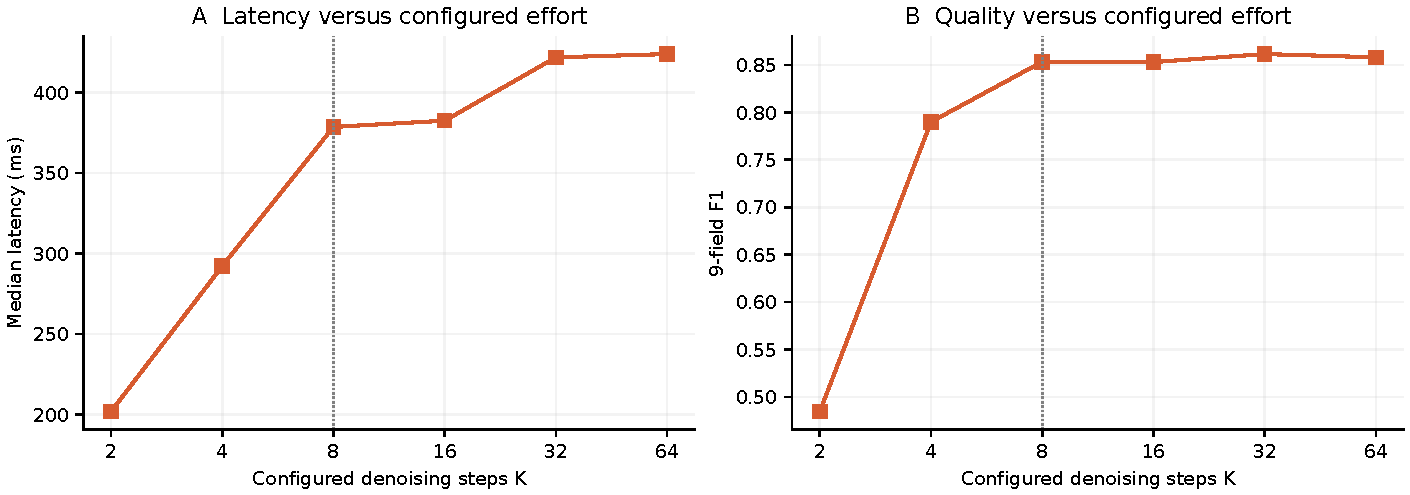
\includegraphics[width=0.85\linewidth]{figures/fig4_ksweep.pdf}
\caption{DG denoising-step sweep (BGL, $n{=}200$, output budget
\canvasLength). Latency is nonlinear in configured $K$. The observed
quality gains become small around $K{=}8$ in this sweep; that is a
practical operating-point choice, not a universal saturation threshold.}
\label{fig:ksweep}
\end{figure}
